% Tipo di documento. L'uso di twoside implica che i capitoli inizino sempre con la prima pagina a sinistra, eventualmente lasciando una pagina vuota nel capitolo precedente. Se questa cosa non va bene, è possibile rimuoverlo. 
\documentclass[a4paper, twoside,openright]{report}
% Dimensione dei margini
\usepackage[a4paper,top=3cm,bottom=3cm,left=3cm,right=3cm]{geometry} 
% Dimensione del font
\usepackage[fontsize=13pt]{scrextend}

% Lingua del testo
\usepackage[english,italian]{babel}
% Lingua per la bibliografia
\usepackage[fixlanguage]{babelbib}
% Codifica del testo
\usepackage[utf8]{inputenc} 
% Encoding del testo
% \usepackage[T1]{fontenc}
% Permette di generare testo fittizio. Mi è stato utile 
% per capire quale sarebbe stata l'impostazione del 
% testo nella pagina prima che scrivessi un determinato paragrafo
% \usepackage{lipsum}
% Per ruotare le immagini
\usepackage{rotating}
% Per modificare l'header delle pagine 
\usepackage{fancyhdr}               

% Librerie matematiche
\usepackage{amssymb}
\usepackage{amsmath}
\usepackage{amsthm}         

% Uso delle immagini
\usepackage{graphicx}
% Uso dei colori
\usepackage[dvipsnames]{xcolor}         
% Uso dei listing per il codice
\usepackage{listings}    
\usepackage{nameref}

\usepackage{float}

% Definizioni per JavaScript
\lstdefinelanguage{JavaScript}{
  keywords={break, case, catch, continue, debugger, default, delete, do, else, false, finally, for, function, if, in, instanceof, new, null, return, switch, this, throw, true, try, typeof, var, void, while, with,let, const},
  morecomment=[l]{//},
  morecomment=[s]{/*}{*/},
  morestring=[b]',
  morestring=[b]",
  morestring=[b]`,
  ndkeywords={class, export, boolean, throw, implements, import, this},
  keywordstyle=\color{blue}\bfseries,
  ndkeywordstyle=\color{darkgray}\bfseries,
  identifierstyle=\color{black},
  commentstyle=\color{purple}\ttfamily,
  stringstyle=\color{red}\ttfamily,
  sensitive=true
}

\lstset{
   language=JavaScript,
   backgroundcolor=\color{white},
   extendedchars=true,
   basicstyle=\footnotesize\ttfamily,
   showstringspaces=false,
   showspaces=false,
   numbers=none,
   tabsize=2,
   breaklines=true,
   showtabs=false,
   captionpos=b,
   frame=single
}
% Per inserire gli hyperlinks tra i vari elementi del testo 
\usepackage{hyperref}     
% Diversi tipi di sottolineature
\usepackage[normalem]{ulem}

% -----------------------------------------------------------------

% Modifica lo stile dell'header
\pagestyle{fancy}
\fancyhf{}
\lhead{\rightmark}
\rhead{\textbf{\thepage}}
\fancyfoot{}
\setlength{\headheight}{12.5pt}

% Rimuove il numero di pagina all'inizio dei capitoli
\fancypagestyle{plain}{
  \fancyfoot{}
  \fancyhead{}
  \renewcommand{\headrulewidth}{0pt}
}

% Stile del codice
\lstdefinestyle{codeStyle}{
    % Colore dei commenti
    commentstyle=\color{teal},
    % Colore delle keyword
    keywordstyle=\color{Magenta},
    % Stile dei numeri di riga
    numberstyle=\tiny\color{gray},
    % Colore delle stringhe
    stringstyle=\color{violet},
    % Dimensione e stile del testo
    basicstyle=\ttfamily\footnotesize,
    % newline solo ai whitespaces
    breakatwhitespace=false,     
    % newline si/no
    breaklines=true,                 
    % Posizione della caption, top/bottom 
    captionpos=b,                    
    % Mantiene gli spazi nel codice, utile per l'indentazione
    keepspaces=true,                 
    % Dove visualizzare i numeri di linea
    numbers=left,                    
    % Distanza tra i numeri di linea
    numbersep=5pt,                  
    % Mostra gli spazi bianchi o meno
    showspaces=false,                
    % Mostra gli spazi bianchi nelle stringhe
    showstringspaces=false,
    % Mostra i tab
    showtabs=false,
    % Dimensione dei tab
    tabsize=2
} \lstset{style=codeStyle}

% Stile di codice per dimensioni maggiori, in cui ho avuto bisogno di un testo più piccolo (ad esempio se si vuole inserire del codice che ha linee molto lunghe). Per usare questo stile piuttosto che il precedente, usare 

% \lstset{style=longBlock}
%  % inserire il codice...
% \lstset{style=codeStyle}

% Il secondo comando consente di tornare allo stile precedente 
\lstdefinestyle{longBlock}{
    commentstyle=\color{teal},
    keywordstyle=\color{Magenta},
    numberstyle=\tiny\color{gray},
    stringstyle=\color{violet},
    basicstyle=\ttfamily\scriptsize,
    breakatwhitespace=false,         
    breaklines=true,                 
    captionpos=b,                    
    keepspaces=true,                 
    numbers=left,                    
    numbersep=5pt,                  
    showspaces=false,                
    showstringspaces=false,
    showtabs=false,                  
    tabsize=2
} \lstset{style=codeStyle}

% Togliendo il commento al comando che segue, si inseriscono nella bibliografia anche le fonti presenti in Bibliography.bib ma non citati direttamente con il comando \cite
% \nocite{*}

% Margini prima e dopo blocchi di codice, per avere più distanza
\lstset{aboveskip=20pt,belowskip=20pt}

% Modifica dello stile dei riferimenti, con il testo in nero
\hypersetup{
    colorlinks,
    linkcolor=black,
    citecolor=black
}

% Aggiunti definizioni, teoremi, linea e listing
\newtheorem{definition}{Definizione}[section]
\newtheorem{theorem}{Teorema}[section]
\providecommand*\definitionautorefname{Definizione}
\providecommand*\theoremautorefname{Teorema}
\providecommand*{\listingautorefname}{Listing}
\providecommand*\lstnumberautorefname{Linea}

\raggedbottom

%\newcommand{\cgs}[1]{{\textcolor{brown}[\textcolor{red}{\bf{GS: }}{ \textcolor{brown}{#1]}}}}             
%\newcommand{\cmc}[1]{{\textcolor{blue}[\textcolor{magenta}{\bf{MC: }}{ \textcolor{blue}{#1]}}}}

% ----------------------------------------------------------------

\setlength{\parskip}{\baselineskip}%
\setlength{\parindent}{0pt}%

% -----------------------------------------------------------------
% Comandi per il color coding delle correzioni
\newcommand{\torevise}[1]{\textcolor{red}{#1}}
\newcommand{\edit}[1]{\textcolor{NavyBlue}{#1}}
\newcommand{\approved}[1]{\textcolor{black}{#1}}

% Comandi per il color coding delle note e delle parti da sistemare
\newcommand{\tomodify}[1]{\textcolor{purple}{#1}}
\newcommand{\note}[1]{\textcolor{Bittersweet}{#1}}

% comandi per il codice inline
\newcommand{\jscode}[1]{\lstinline[language=JavaScript]{#1}}
\newcommand{\htmlcode}[1]{\lstinline[language=HTML]{#1}}

% Profondità della ToC
\setcounter{tocdepth}{2}

% Abbreviazioni per i comandi
\newcommand{\n}{\newline}
\newcommand{\nl}{\newline \newline }
% -----------------------------------------------------------------
\begin{document}


\begin{titlepage}
\begin{figure}[!htb]
    \centering
    
\includegraphics[keepaspectratio=true,scale=0.5]{images/Frontespizio/cherubinFrontespizio.eps}
\end{figure}

\begin{center}
    \LARGE{UNIVERSITÀ DI PISA}
    \vspace{5mm}
    \\ \large{DIPARTIMENTO DI INFORMATICA}
    \vspace{5mm}
    \\ \LARGE{Laurea Triennale in Informatica}
\end{center}

\vspace{15mm}
\begin{center}
    {\LARGE{\bf Live LG:\\ \vspace{5mm} 
    app per sistemi IoT, Video e Smart TV di distribuzione contenuti multimediali targettizzati.
    }}
\end{center}
\vspace{30mm}

\begin{minipage}[t]{0.47\textwidth}
	{\large{Relatore:}{\normalsize\vspace{3mm}
	\bf\\ \large{Prof.sa: Laura Semini} \normalsize\vspace{3mm}\bf \\ \large{Matteo Baldi}}}
\end{minipage}
\hfill
\begin{minipage}[t]{0.47\textwidth}\raggedleft
	{\large{Candidato:}{\normalsize\vspace{3mm} \bf\\ \large{Lorenzo Arcidiacono}}}
\end{minipage}

\vspace{30mm}
\hrulefill
\\\centering{\large{ANNO ACCADEMICO 2021/2022}}

\end{titlepage}
\include{chapters/Abstract}
\section*{Ringraziamenti}

Non so nemmeno da dove iniziare, vorrei ringraziare ogni persona che ho avuto accanto in tutto questo (lungo) percorso, tutti quelli che hanno festeggiato un esame con me, quelli che la notte prima di ogni esame erano seduti sul gradino davanti all'Orzo con una birra in mano e tutti quelli che mi hanno spronato nei momenti in cui ho pensato di mollare.

Vorrei poter ringraziare i miei nonni che avrei voluto accanto a me oggi. Perché loro, che di computer non ci hanno mai capito nulla, sono stati i primi a chiedere consiglio a me quando avevano un bisogno.

Ringrazio mio padre che sin da piccolo mi ha aiutato a coltivare questa mia passione obbligando mamma a non usare il telefono in modo che io potessi andare online (che meraviglia la 56K). Lo ringrazio per tutte quelle parole non dette ma che in qualche modo è riuscito a farmi capire.

Ringrazio mia madre che mi sopporta ogni giorno, che con i suoi piccoli gesti riesce sempre a farmi stare meglio, che mi ha regalato un po' della sua empatia e che, insieme a papà, mi ha sempre spinto a inseguire i miei sogni sapendo di avere una rete nel caso in cui fossi caduto.

Ringrazio mia sorella che spero sia orgogliosa di me almeno quanto lo sono di lei. Per aver sempre cercato di vedere il meglio di me e di farlo vedere anche a me.

Vorrei ringraziare Andrea, Stefano, Leonardo, Giulia, Simone e tutte le persone che ho incontrato nel mio cammino come scout per avermi sempre dato una scusa valida per non studiare ma anche per tutte le serate davanti a un fuoco o a una birra, per avermi fatto sentire leggero anche nei periodi in cui mi sentivo a terra, per ogni nota suonata e stonata insieme e per ogni riunione infinita che grazie a voi riusciva ad essere comunque un momento di svago.

Vorrei ringraziare il Dott. Guerri che mi ha aiutato a ritrovare un pezzo di me che avevo perso da tempo.

Ringrazio i miei colleghi, in particolare Ruggero e Aldo, che mi hanno supportato durante il tirocinio, mi hanno dato fiducia e mi sopportano ancora. 

Ringrazio Fede, per essermi stata accanto in alcuni momenti difficili, per sopportarmi ogni giorno (anche quando non mi sopporto da solo), per farmi sentire sempre leggero e per tutte le risate che è riuscita a strapparmi in ogni occasione.

Ringrazio la Professoressa Semini per l'aiuto datomi durante il tirocinio e la stesura di questa relazione nonostante i miei ritardi e le consegne notturne.

Vorrei ringraziare quei professori che sono riusciti a passarmi la passione per la loro materia e a lasciarmi insegnamenti che ancora oggi mi risuonano in testa.

Ultimo vorrei ringraziare il mio coinquilino da 2 anni, che sopporta le mie giornate no e i miei momenti di nervosismo e che al ritorno da ogni esame mi ha aspettato scodinzolante (un po' perché gli fa piacere vedermi e un po' per avere un biscottino).

Non sono bravo a scrivere e sono anche peggio ad aprirmi, quindi alcune cose possono essere suonate un po' banali o vuote ma spero che sappiate quanto ci tengo a voi.
\tableofcontents


\chapter{Introduzione} 
% \note{levare capitolo 1 come titolo}
\linespread{1.5}

\section{In Breve}
Breve introduzione sullo scopo e svolgimento del tirocinio compreso il contesto in cui ho svolto il lavoro, sull'applicazione Livesignage e sua architettura, sullo stato dell'arte e sugli obiettivi raggiunti. Infine una descrizione della struttura di questa relazione.

\section{Scopo del tirocinio}

\edit{Il tirocinio è stato svolto presso l'azienda Softhrod srl. di Volterra all'interno del progetto Livesignage, un'applicazione focalizzata sulla distribuzione di contenuti multimediali targettizzati. Lo scopo del tirocinio è l'analisi, la progettazione e lo sviluppo di un'applicazione lato client per il sistema operativo WebOs Signage sui dispositivi LG:  display professionali, videowall, smart TV, sistemi IoT, media player. L'applicazione deve essere in grado di mostare specifici contenuti multimediali sulla base di eventi acquisiti dall'ambiente circostante, come ad esempio condizioni metereologiche o orario, e parametri indicati dall'utente. L'applicazione è stata sviluppata in linguaggio Javascript sfruttando le API REST messe a disposizione dal sistema operativo.}

\section{Modalità di lavoro}

Ho lavorato in modalità mista ( telematica e presenza ) in maniera prevalentemente autonoma, ma mantenendo un confronto diretto sia con gli altri sviluppatori sia con i designer per tutte le scelte riguardanti le logiche e lo sviluppo dell'applicazione. Ho così avuto modo di capire quale sia il processo produttivo dell'azienda, come si lavora in team e l'attenzione per l'esperienza utente, fondamentale per questo ambito.

\section{Digital signage e Livesignage}

\edit{Il digital signage è una forma di comunicazione direttamente nel punto vendita, in spazi pubblici aperti o all'interno di edifici, anche nota in Italia come segnaletica digitale, videoposter o cartellonistica digitale, i cui contenuti vengono mostrati ai destinatari attraverso schermi elettronici o videoproiettori disposti in maniera strategica. Le tipologie di contenuti che possono essere mostrati sono molteplici: video, mappe, immagini, menù, feed real time, elementi interattivi; di conseguenza sono molteplici i contesti in cui può essere utilizzato: negozi, ristoranti, alberghi e totem nelle città sono alcuni esempi.}

Livesignage è un’applicazione per il digital signage sviluppata per vari dispositivi specializzati tra i quali quelli di Samsung. \edit{L’idea è quella di fornire all'utente un modo semplice e flessibile per creare i propri contenuti cercando, quando possibile, di automatizzare il processo usando tutte le informazioni contenute sul suo sito web o sul proprio database}. Tramite l'utilizzo di alcuni plugin, è possibile ampliare ancora le feature disponibili: come la possibilità di fare webcall e l'integrazione delle informazioni reperibili dai propri social network.

\edit{Inoltre, alla creazione di una playlist (vedi sezione \ref*{statoarte}), viene automaticamente creata una progressive Web App: un'applicazione navigabile direttamente dal browser e completamente impostabile dal creatore dei contenuti permettendo un'interazione maggiore dell'utente finale.}

\edit{Nella Figura \ref{fig:liveToursitSample} viene mostrato un esempio di quello che potrebbe essere mostrato su un totem installato in una città; tramite il codice QR creato automaticamente insieme ai contenuti mostrati, il consumatore può quindi ricevere le informazioni in modo più dettagliato sul proprio dispositivo mobile senza bisogno di scaricare applicazioni o fare ricerche online.}

\begin{figure}[!htb]
    \centering
    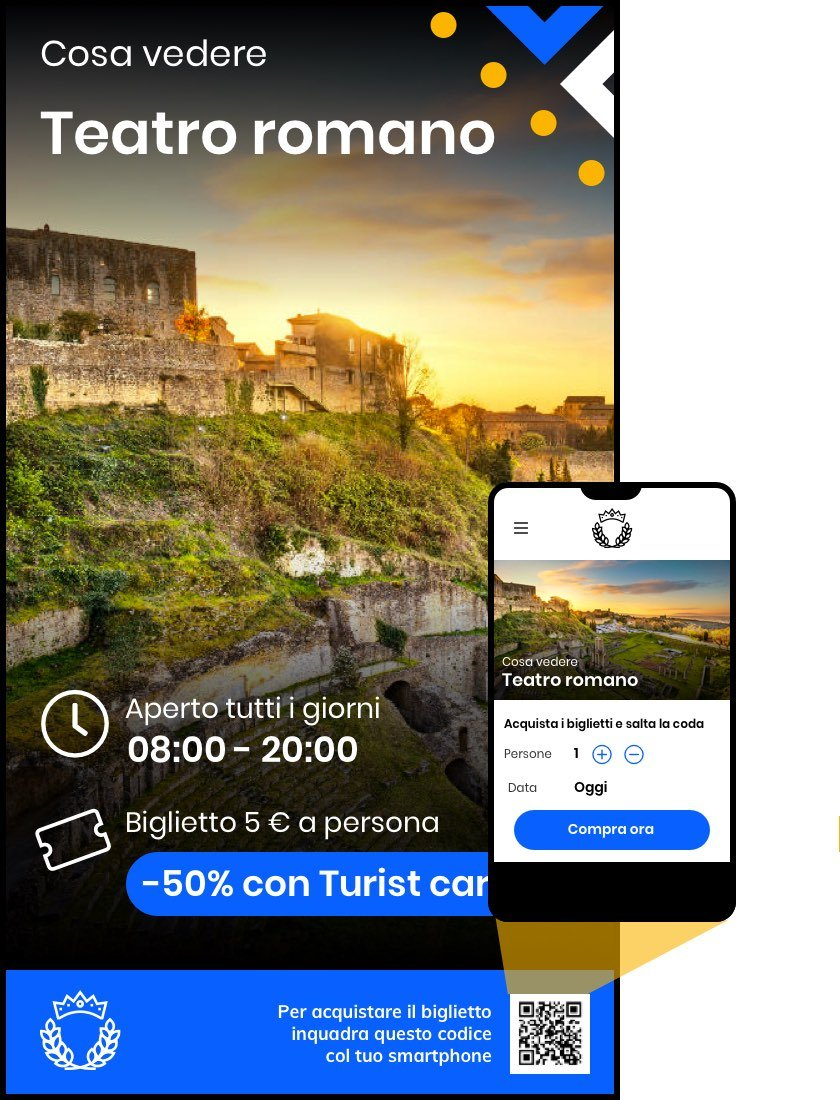
\includegraphics[width= 0.5\textwidth]{images/Introduzione/LiveTurist.jpg} 
    \caption{Esempio di infografica in un'installazione cittadina.} 
    \label{fig:liveToursitSample}
\end{figure}



\section{Stato dell'arte}\label{statoarte}

All'inizio del tirocinio il client di Livesignage era già disponibile per dispositivi di Samsung e Raspberry.  

L'idea alla base dell'applicazione è quella di mostrare una serie di slide organizzate in playlist; ogni slide può mostrare diversi tipi di contenuti come ad esempio immagini, video, web page, mappe, notizie, input esterni (ad esempio telecamere e fogli di calcolo). Le playlist possono essere di diverso tipo:

\begin{itemize}
    \item Semplici: le slide vengono mostrate a schermo intero e si susseguono continuamente;
    \item Composte: in questo caso lo spazio a disposizione viene suddiviso in più parti e in ognuna di queste viene mostrata una playlist diversa (Fig. \ref*{fig:playlist-composta});
    \item Concatenate: vengono concatenate più playlist una dopo l'altra.
    \begin{figure}[!htb]
        \centering
        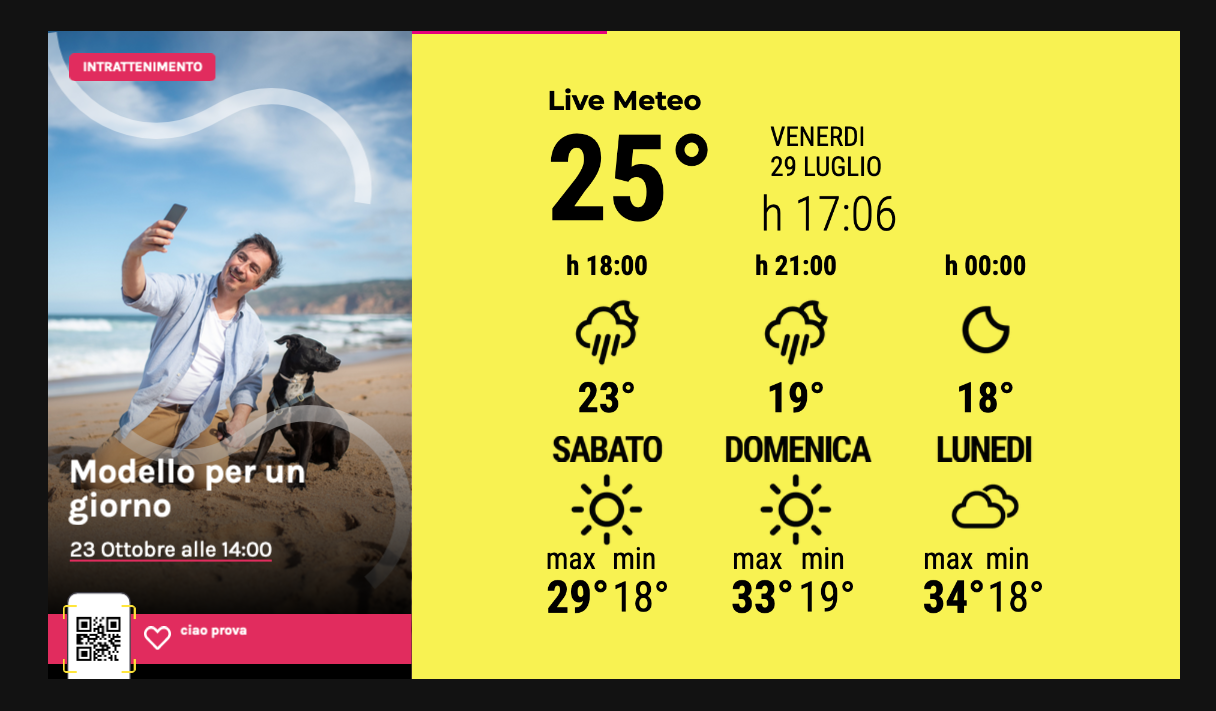
\includegraphics[width= 0.8\textwidth]{images/Introduzione/playlist-composta.png} 
        \caption{Una playlist composta.} 
        \label{fig:playlist-composta}
    \end{figure}
\end{itemize}


Oltre alle playlist è possibile utilizzare dei plugin per poter dare al cliente più possibilità di personalizzazione. Ad esempio permettendo di  mostrare contenuti interattivi utilizzando l'input dell'utente tramite il touchscreen o di inserire il proprio e-commerce.

\subsection{Architettura}
\begin{figure}[!htb]
    \centering
    \includegraphics[width= 0.8\textwidth]{images/Introduzione/architettura.jpg} 
    \caption{Architettura dell'applicazione.} 
    \label{fig:architettura}
\end{figure}

\edit{L'applicazione è suddivisa in due parti: una parte è installata sul dispositivo per il digital signage, questa si occupa di riceve dal back office le playlist da mostrare e le impostazioni che il creatore di contenuti ha impostato (timer di accensione, volume, luminosità), la seconda parte è online ed è accessibile tramite una web page (Fig: \ref*{fig:schermata-web}): qui è possibile controllare alcune funzioni del device client, creare e impostare le proprie playlist e i plugin. 
\nl
Le modifiche impostate dal back office vengono comunicate al dispositivo che, tramite le interfacce offerte dal sistema, scrive i file necessari alla persistenza delle informazioni, scarica i contenuti multimediali necessari e configura le impostazioni selezionate.}


La figura \ref*{fig:architettura} mostra in maniera schematica l'architettura dell'applicazione e l'interazione con il consumatore.

\begin{figure}[!htb]
    \centering
    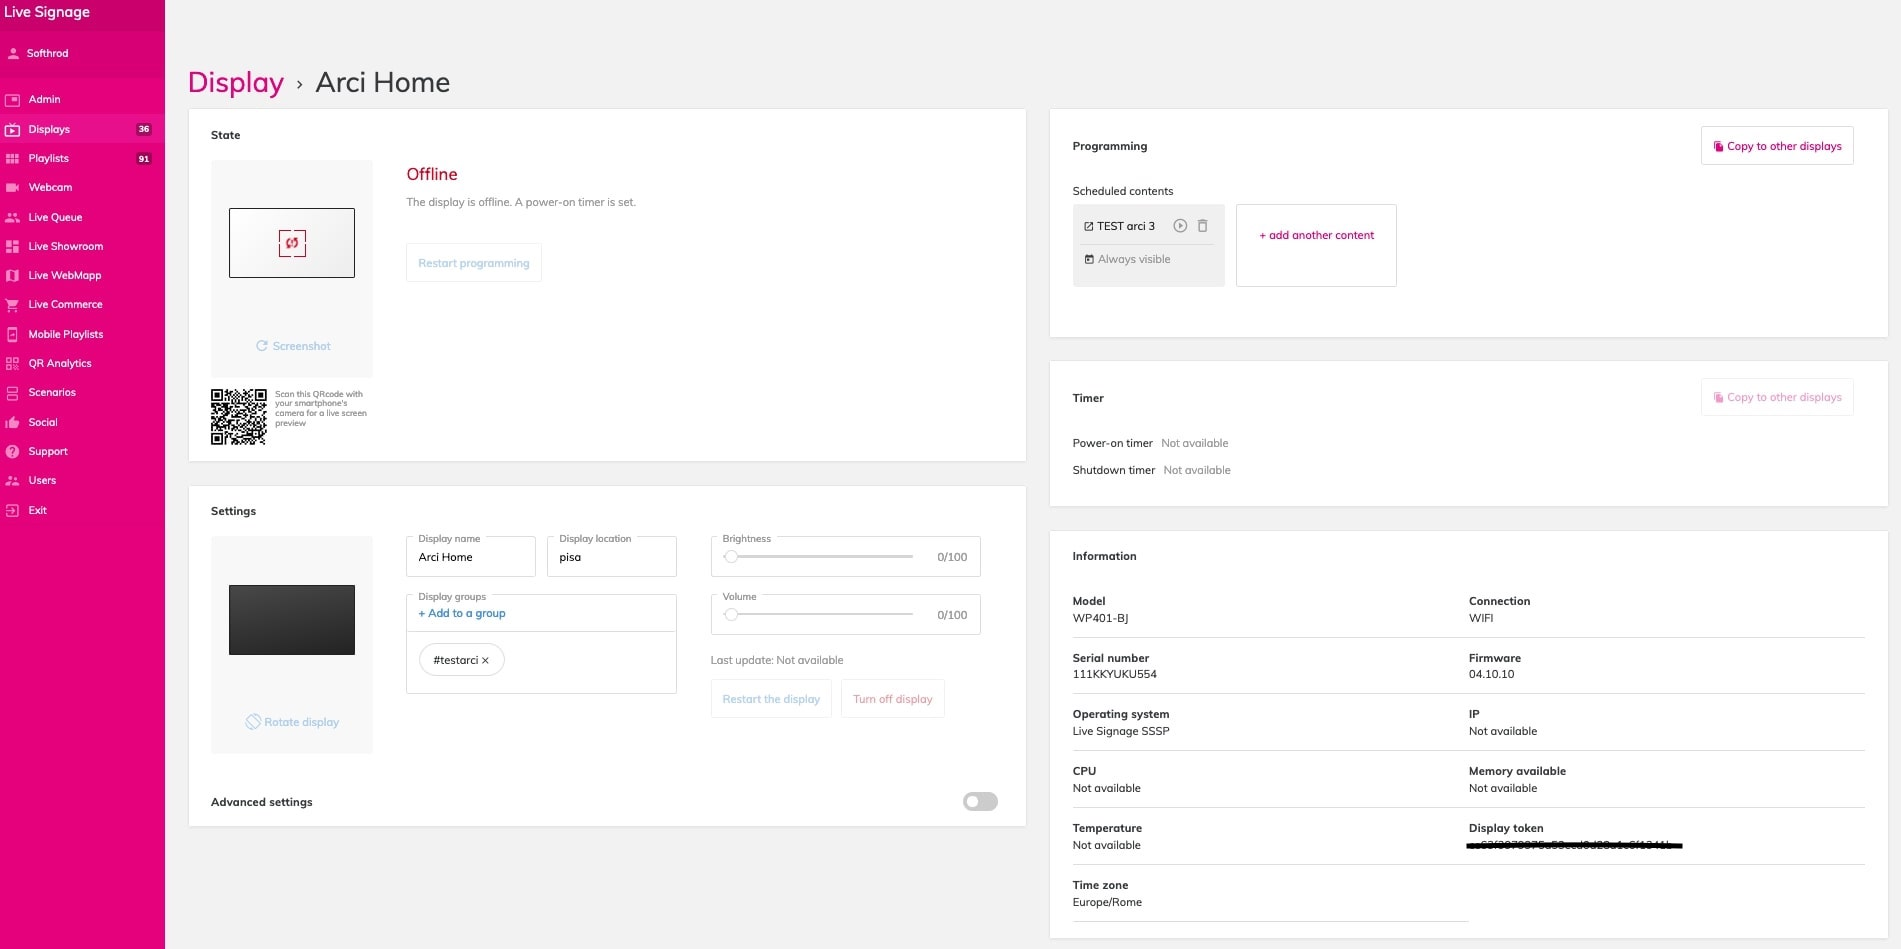
\includegraphics[width= 1.1\textwidth]{images/Introduzione/SchermataWebLS.jpg} 
    \caption{Schermata della Web Page per programmare il display.} 
    \label{fig:schermata-web}
\end{figure}
% \note{figura web page piú grande}

\section{Requisiti}
\edit{Lo svolgimento del lavoro è incentrato sullo sviluppo di un'applicazione client per il sistema operativo WebOS signage di LG; questa deve essere in grado di mostrare contenuti multimediali tramite l'uso di HTML e CSS su un web engine basato su Chromium, deve poter eseguire degli script JavaScript e comunicare con il device tramite l'uso delle interfacce messe a disposizione dal sistema operativo.
L'applicazione deve inoltre poter salvare in memoria i contenuti e le informazioni necessarie affinchè possa funzionare anche in assenza di connessione.} 

\section{Obiettivi raggiunti}

Al termine del tirocinio la versione di Livesignage per WebOS Signage è stata correttamente sviluppata; ho avuto inoltre modo di aggiungere, o almeno studiare la possibilità di farlo, alcune funzionalità non presenti nella versione per dispositivi Samsung. \edit{Queste non erano previste a inizio tirocinio ma sono state pensate a seguito dello studio della documentazione.}

\section{Struttura della relazione}
Di seguito una breve descrizione della suddivisione in capitoli di questa relazione.
\begin{itemize}
    \item Tecnologie utilizzate: Descrizione delle tecnologie a disposizione, loro differenze e scelte implementative da queste derivanti. Linguaggi e librerie utilizzate.
    \item Livesignage su WebOs: Descrizione del lavoro svolto, difficoltà incontrate e soluzioni trovate, modifiche all'applicazione pre-esistente. Descrizione della fase di testing finale.
    \item Studio di funzionalità aggiuntive: In questo capitolo si presenta una descrizione della fase di analisi e, quando possibile, aggiunta delle nuove funzionalità e alcune idee per possibili miglioramenti futuri.
    \item Conclusioni: Riassunto dei punti principali affrontati e degli obiettivi raggiunti. Competenze acquisite.
\end{itemize}
\chapter{Tecnologie utilizzate}

\section{In breve}
Descrizione delle tecnologie a disposizione (due device diversi), loro differenze e scelte implementative da queste derivanti. Linguaggi e librerie utilizzate. 

\section{Dispositivi a disposizione}
Per lo svolgimento del tirocinio sono stati messi a disposizione due device LG con versioni differenti del sistema operativo:
\begin{itemize}
    \item Un player (un device non dotato di schermo) con la versione 4.0;
    \item Un professional display con la versione 6.0.
\end{itemize}

Oltre alle differenze hardware i due modelli presentano importanti differenti al livello del software; sul primo è installato il web engine Chromium 53 e supporta solamente la visualizzazione di 2 video contemporaneamente, il secondo supporta fino a 4 video e ha installato Chromium 79.

La differenza di web engine ha comportato un'analisi approfondita delle librerie e delle funzioni JavaScript supportate e ha quindi guidato le scelte implementative del progetto.


\section{Linguaggi di programmazione e librerie} \label{linguaggi}

Il tirocinio, oltre al linguaggio di markup HTML e quello di stile CSS, si è basato sul linguaggio di programmazione JavaScript: un linguaggio interpretato usato principalmente nella programmazione front-end delle pagine web (la cui documentazione è reperibile in \cite{MdN}).

Oltre alle librerie di sistema (vedi \ref{api}), sono state utilizzate la librerie JQuery \cite{jQDoc} per la manipolazione delle pagine HTML e per la gestione degli eventi e la libreria Dixie.js \cite{dixie} per la gestione dei database (descritti in \ref*{database}). Entrambe le librerie sono già utilizzate negli altri client sviluppati dall'azienda ed è stato quindi deciso di mantenerle sia per una questione di manutenibilità dei diversi client, sia perché comportano notevoli miglioramenti alla leggibilità del codice e al suo funzionamento.

Non avendo familiarità con i linguaggi e le tecnologie utilizzati si è reso necessario un'iniziale studio approfondito dei linguaggi e delle librerie necessarie.

\subsection{Scelta delle API} \label{api}

Dal momento che il linguaggio Javascript, per questioni di sicurezza, non ha modo di comunicare con il sistema operativo sottostante in modo nativo, sono state messe a disposizione, dagli sviluppatori LG, delle interfacce implementate sottoforma di librerie Javascript per poter eseguire operazioni e ricevere informazioni dal device quali: informazioni di rete, stato del dispositivo, eventuali timer di accensione e spegnimento e gestione degli aggiornamenti dell'applicazione e del sistema operativo.

I set di API (Application Programming Interface) messi a disposizione sono molteplici (come specificato in \cite{LgDoc}), tuttavia non tutti sono compatibili con tutte le versioni del sistema operativo. È stato quindi deciso di basare il progetto sul set SCAP (Signage Application Platform) API v1.8 poiché questo è supportato dalla maggior parte dei dispositivi LG in commercio. Alcune di queste interfacce saranno approfondite nel capitolo \ref*{svolgimento}.

Non tutte le API messe a disposizione sono state utilizzate durante lo svolgimento del tirocinio, è stata comunque fatta un'analisi al fine di capire quali possano essere di interesse per implementazioni successive (vedi \ref*{future_implementazioni}).
\chapter{Livesignage su WebOS}\label{svolgimento}
\section{In Breve}
Descrizione del lavoro svolto: portare l'applicazione già esistente per i dispositivi Samsung sui dispositivi LG, difficoltà incontrate e soluzioni trovate, modifiche all'applicazione pre-esistente. Descrizione della fase di testing finale.

\section{Fase di analisi}

Nelle prime fasi del tirocinio il lavoro ha riguardato l'analisi dell'applicazione preesistente, della documentazione delle interfacce messe a disposizione da LG e lo studio dei linguaggi di programmazione utilizzati (vedi \ref*{linguaggi}).

Nella Fig.\ref*{fig:architettura_2} è presentato uno schema dell'architettura dell'applicazione lato client e lato server in cui sono mostrate le componenti principali: Livesignage, il sistema operativo e il web server che ospita il back office.

\begin{figure}[!htb]
    \centering
    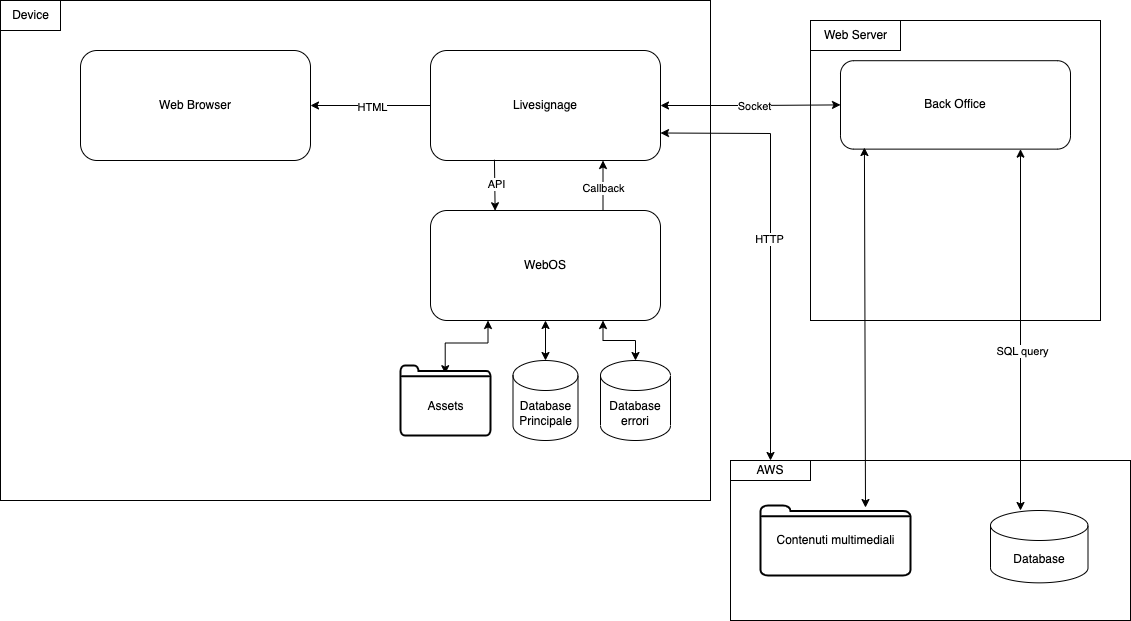
\includegraphics[width= 1\textwidth]{images/svolgimento/webos_client_archi.png} 
    \caption{Architettura del client e dei componenti con cui comunica.} 
    \label{fig:architettura_2}
\end{figure}

\begin{itemize}
    \item Web server: qui vengono salvati in un database MySQL tutte le informazioni degli utenti, dei dispositivi e le playlist create: tutte queste informazioni vengono elaborate e inviate ai client attraverso una socket. Questo si occupa inoltre di salvare su AWS le immagini e i video caricati dal creatore di contenuti in modo da essere scaricabili tramite link dai device client;
    \item Livesignage: dopo aver stabilito il canale di comunicazione con il web server, resta in attesa dei messaggi da questo inviati e si occupa di svolgere le operazioni richieste tramite back office dal creatore di contenuti, comunicando, tramite le API a disposizione, con il sistema operativo sottostante.
    \item Sistema operativo: gestisce le richieste fatte da Livesignage tramite API, una volta che queste sono portate a termine chiama le funzioni di callback passate come parametri delle interfacce (vedi \ref*{apicode}).
\end{itemize}

Gli altri componenti del sistema sono: il database principale su cui viene salvato il codice HTML delle playlist, il database dei log in cui sono scritti i messaggi di errore, in modo che siano successivamente scaricabili dal creatore di contenuti e la cartella degli assets nella quale vengono salvate le immagini e i video delle playlist create, in modo che queste possano essere visualizzate anche offline.

\subsection{Codice Livesignage}

\subsubsection{Suddivisione del codice}

Nella cartella principale sono presenti 3 file HTML: 
\begin{itemize}
    \item index.html: è la prima pagina ad essere caricata e si occupa di chiamare le funzioni JavaScript per controllare se il device sia stato precedentemente associato a Livesignage.
    \item noAssociation.html: questa pagina viene caricata nel caso che il dispositivo non sia associato e mostra un codice univoco per l'associazione.
    \item display.html: questa è la pagina in cui viene iniettato il codice delle playlist e dei plug-in.
\end{itemize}

Il resto dei file fondamentali si trova nella cartella \jscode{js/}, qui sono raccolti gli script e le classi necessarie al corretto funzionamento dell'applicazione:

\begin{itemize}
    \item association.js: classe che controlla e gestisce l'associazione del device;
    \item connection.js: i metodi di questa classe vengono chiamati ciclicamente per verificare lo stato della connessione;
    \item db.js: classe che si occupa della gestione del database principale, verrà vista in maniera più approfondita ( insieme a dblog.js ) in \ref*{database};
    \item dblog.js: qui è contenuta la gestione del database degli errori;
    \item display.js: in questa classe sono definiti i metodi che implementano la comunicazione con il sistema operativo attraverso le API. Alcune di queste implementazioni verranno approfondite in \ref*{js_code};
    \item filemanager.js: si occupa della gestione del file system del sistema e del download e della cancellazione degli assets;
    \item livesignage.js: in questa classe sono contenuti i metodi per la visualizzazione delle playlist, la gestione di alcuni comandi ricevuti dal server come: il cambio di slide, il passaggio alla visualizzazione dell'ingresso HDMI e le richieste di salvataggio e cancellazione delle playlist dal database;
    \item log.js: qui sono presenti i metodi per la creazione dei messaggi di errore e l'invio di questi al back office in modo che possano essere visualizzati dal cliente;
    \item main.js: questo è lo script principale che si occupa di chiamare le altre classi, in particolare controlla se sia necessario scaricare un aggiornamento dell'applicazione o del firmware del sistema operativo (vedi \ref*{update}), chiama a intervalli di tempo prestabililti i metodi per il controllo della connessione, invoca i metodi che si occupano della comunicazione con il back office e, se il display risulta offline, avvia la visualizzazione dell'ultima playlist salvata;
    \item monitor.js: questa classe si occupa di aprire la socket verso il back office e di restare in ascolto su questa, alla ricezione dei messaggi chiama i metodi necessari;
    \item speedtest.js: questa classe viene invocata quando si riceve una richiesta per valutare lo stato della rete dal back office.
\end{itemize}

\subsection{Documentazione WebOS Signage}\label{WebOS_doc}

Dopo l'analisi dell'applicazione preesistente è stata studiata la documentazione (disponibile in \cite{LgDoc}) dei dispositivi LG.

Come detto in \ref*{api} sono state analizzate le diverse interfacce messe a disposizone dal sistema per la comunicazione tra il browser e il sistema operativo; le librerie disponibili sono: 
\begin{itemize}
    \item SCAP API: un set di interfacce specifiche per WebOS Signage, la versione di WebOS dedicata ai sistemi di digital signage,suddivise in diverse classi a seconda delle funzionalità. Questo è il set scelto per lo sviluppo poiché, sebbene non sia il più recente, è l'unico compatibile con tutti i device di digital signage di LG e che abbia un set ampio di interfacce tale da coprire i requisiti dell'applicazione;
    \item IDCAP API: è il nuovo standard di API di LG che ha come obiettivo quello di rendere univoche le interfacce per le diverse versioni di WebOS, sia quella per il digital signage che quella per le TV commerciali. Nonostante questo set sia quello raccomandato da LG è supportato solamente da WebOS Signage 6.0 e successivi;
    \item Harmony API: una libreria, specifica per WebOS Signage, contenente le interfacce per la comunicazione con alcuni dispositivi esterni come ad esempio stampanti, sensori NFC e infrarossi;
    \item CustomJS API: questo set aggiunge alcune interfacce mancanti alla libreria SCAP. Questa libreria è aggiunta all'applicazione sviluppata al fine di espanderne le funzionalità (si veda \ref*{aggiunte}).
\end{itemize}

Sono state anche studiate le caratteristiche hardware e software dei dispositivi, cercando di capire quali fossero quelle minime comuni a tutti. Dal momento che le componenti software e hardware sono molto diverse tra loro a seconda della versione del sistema operativo, sono stati presi in considerazione solo i dispositivi che supportano almeno WebOS Signage 4.0. Di seguito sono riportate le specifiche e le versioni dei linguaggi di programmazione supportate che sono state identificate dopo l'analisi.

\begin{center}
\begin{tabular}{ |l|r| } 
     \hline
     HTML & versione 5 \\ 
     CSS & versione 3 \\ 
     JavaScript & versione 1.6+ \\ 
     \hline
     Web Engine & Chrome 53 \\ 
     HTTP, HTTPS & \checkmark \\ 
     XMLHttpRequest (AJAX) & \checkmark \\ 
     JSON & \checkmark \\ 
     \hline
     RAM & 2.0 GB \\
     Memoria & 8.0 GB\\
     Risoluzione & 1920x1080\\
     \hline
\end{tabular}
\end{center}

\section{Scrittura delle classi JavaScript}\label{js_code}

\subsection{Codice delle chiamate alle API} \label{apicode}
Le chiamate API per i dispositivi LG sono di due tipi: le prime ( Listing \ref*{lst:apiget} ) servono per chiedere delle informazioni al sistema operativo come ad esempio il numero seriale, il MAC address o il livello del volume, le seconde (Listing \ref*{lst:apipost}) servono per modificare delle impostazioni di sistema come il volume, lo stato del dispositivo (accensione e spegnimento) o la rotazione dello schermo. In entrambi i casi vengono passate due funzioni dette di callback che saranno eseguite in caso di successo o fallimento della chiamata; le chiamate di modifica del device necessitano inoltre di una struttura contenente i nuovi valori da impostare.

In risposta viene passato un oggetto alle funzioni di callback, in Listing \ref*{lst:returnsample} vengono mostrati due esempi: uno in caso di successo, uno di fallimento.

\lstinputlisting[caption={Esempio chiamata API WebOS.}, label={lst:apiget}, language=JavaScript, firstline=0, lastline=18]{listings/svolgimento/api_sample.js}
\lstinputlisting[caption={Esempio chiamata API WebOS.}, label={lst:apipost}, language=JavaScript, firstline=37, lastline=54]{listings/svolgimento/api_sample.js}
\lstinputlisting[caption={Esempi dei messaggi di risposta.}, label={lst:returnsample}, language=JavaScript, firstline=20, lastline=34]{listings/svolgimento/api_sample.js}

Poichè queste funzioni sono asincrone e quindi indipendenti dalla normale esecuzione del codice, è stato necessario gestire l'attesa delle risposte e la sincronizzazione con il resto del codice.

JavaScript non è un linguaggio multi-trhead ma può gestire delle funzioni asincrone tramite un call stack e un event loop che sono parte dell' ambiente di esecuzione JavaScript del browser: il call stack mantiene una coda di tutte le chiamate effettuate dal thread principale, l'event loop si occupa di prendere dalla coda ed eseguire le chiamate asincrone in un ambiente separato dal thread principale; spesso queste funzioni sono interfacce a metodi di basso livello implementati dal web engine in C o C++. In questo modo la funzione successiva nella coda può essere eseguita mentre quella bloccante è eseguita in background. 
Alle funzioni asincrone possono essere passate come parametri una o più funzioni, dette callback, da invocare alla fine dell'esecuzione dell'operazione asincrona; queste saranno inserite nel call stack dall'event loop.  \cite{MdN}.

In Listing \ref*{lst:callbacksample} si può vedere un esempio di queste funzioni: in questo caso la funzione asincrona è \jscode{getNetworkInterface} che si occupa di richiedere al sistema operativo le informazioni riguardanti la connessione, a cui vengono passate \jscode{successCb} e \jscode{failureCb}; alla fine dell'esecuzione dell'operazione asincrona,in caso di successo, verrà inserita nel call stack la funzione \jscode{successCb} e il parametro \jscode{cbObject} sarà l'oggetto contenente i dati ricevuti dal sistema.

\lstinputlisting[caption={Funzioni di callback.}, label={lst:callbacksample}, language=JavaScript]{listings/svolgimento/callback_sample.js}

Si è cercato di ridurre il numero di chiamate alle API, per diminuire in maniera sostanziale i ritardi causati da queste, salvando i dati destinati a perdurare nel tempo nel \jscode{localStorage}, un oggetto definito dal browser che permette di salvare in maniera temporanea delle coppie di oggetti chiave-valore. Tuttavia, non essendo assicurata dal browser la persistenza di questo oggetto, sono stati implementati tutti i controlli necessari. In \ref*{freestorage} saranno evidenziati i problemi relativi alla capacità del localStorage e alle soluzioni trovate al fine di bilanciare la velocità di esecuzione e la disponibilità dello spazio di memoria.

\subsection{Flusso principale}\label{flusso_principale}

La prima funzione invocata al momento dell'avvio è \jscode{start()} definita in \jscode{main.js} che, come prima cosa controlla se sia disponibile un aggiornamento dell'applicazione o del firmware. Una volta scaricata la nuova versione, dopo aver riavviato il dispositivo, la installa; in caso non siano presenti aggiornamenti o il download non sia riuscito, viene inviata una richiesta al server per verificare se il display sia già stato associato o meno. In caso affermativo, riceve le informazioni relative al contenuto da mostrare, altrimenti viene generato dall'applicazione client un codice alfanumerico che identifica il display; questo codice sarà poi inserito dal proprietario del display nel portale online in modo da associarvi il device. Nel caso in cui il display risulti offline all'avvio viene controllato quale sia l'ultimo contenuto salvato sul database e, se disponibile, viene mostrato fino a che non sia possibile collegarsi con il web server e ricevere eventuali nuovi contenuti.


Viene inoltre avviato il controllo a intervalli di tempo prestabiliti, mediante la funzione built-in \jscode{setInterval}, della connessione (Listing \ref*{lst:checkconnection}): viene inviata una richiesta tramite il protocollo HTTP a un URL predefinito e si controlla che questa vada a buon fine (vedi \ref*{connection}).

\lstinputlisting[caption={Controllo dello stato della connesione.}, label={lst:checkconnection}, language=JavaScript]{listings/svolgimento/checkconnection.js}

\section{Cambiamenti di logiche e scelte implementative}

\subsection{Protocollo di comunicazione e gestione della connessione}\label{connection}

Durante il flusso principale viene mantenuta aperta una socket di comunicazione con il web server: su questa vengono ricevuti i messaggi da parte del back office in caso di cambiamenti ai contenuti da mostrare o alle impostazioni del device sia che siano selezionate direttamente dal creatore di contenuti sia se siano dovute ad automazioni predefinite dall'applicazione. Ad esempio è possibile impostare il cambiamento della playlist in base all'orario o al meteo.

La classe \jscode{Monitor} si occupa della gestione della socket e all'arrivo di un messaggio chiama le funzioni da eseguire per portare a termine l'operazione richiesta: in Listing \ref*{lst:monitor} viene mostrata una visione parziale della funzione \jscode{parseMessagge()} che si occupa di tutta la gestione.

\lstinputlisting[caption={parseMessage().}, label={lst:monitor}, language=JavaScript]{listings/svolgimento/monitor.js}

Nel caso in cui la socket venga chiusa, a causa di errori o per mancanza di connessione, il device viene ritenuto offline: si provvede quindi a eliminare momentaneamente i contenuti che necessitano di una connessione attiva ( meteo, notizie, video online) e viene avviato un meccanismo che prova a riaprire la socket ad intervalli di tempo prestabiliti.

A seguito dei test è stato notato che questo protocollo non assicura di accorgersi in maniera tempestiva dell'assenza di rete ed è stato quindi necessario implementare un secondo protocollo, mostrato in \ref*{flusso_principale}, in cui periodicamente viene fatta una chiamata HTTP per controllare che sia presente la connessione.

La necessità di accorgersi velocemente della mancanza di connessione è dovuta alla presenza delle fonti esterne citate sopra che, qualora non abbiano accesso alla rete, possono mostrare errori, dati non aggiornati o addirittura bloccare l'esecuzione dell'applicazione.

\subsection{Lettura e scrittura dei database} \label{database}

Al fine di garantire la corretta visualizzazione dei contenuti in caso di assenza di connessione e per ridurre il numero di chiamate HTTP e conseguenti download degli assets necessari all'arrivo dei dati dal back office: al momento del cambio di una playlist o dell'inserimento di un plug-in, tutti i dati sono salvati in locale su un database non relazionale.

Dal momento che JavaScript non prevede i metodi per la comunicazione con un database SQL, è stata usata la libreria Dixie.js \cite{dixie} che permette di salvare i dati necessari in un file di testo, appositamente formattato, e accederli tramite indicizzazione chiave - valore. Il file viene letto all'avvio dell'applicazione e viene creato il database che sarà quindi accessibile tramite le funzioni della libreria. Il salvataggio del database avviene sovrascrivendo il vecchio file nel file system.

Dixie.js si occupa di creare e leggere le entry nell'\jscode{IndexedDB}, un database NoSQL presente nel web browser. Come il \jscode{localStorage} (vedi \ref*{freestorage}) questo database non assicura la persistenza dei dati ma è pensato, a differenza del primo, per ospitare una grande quantità di dati. La libreria, oltre a facilitare le operazioni di lettura e scrittura, permette di ricreare velocemente la struttura e i dati contenuti nel database al momento dell'ultimo salvataggio.

Durante lo studio della documentazione LG è stato osservato che il buffer di memoria per la lettura e scrittura di un file è solo di 10 KB; è stato quindi necessario implementare le funzioni di scrittura e lettura di un file in maniera ricorsiva in modo che fosse possibile usarla come funzione di callback.
Dal momento che il numero di chiamate necessarie a portare a termine le operazioni è elevato ed i tempi di esecuzione intorno ai 30s, è stato quindi deciso di implementare le due funzioni in modo completamente asincrono rispetto al resto del flusso di esecuzione. 

Nonostante questo, il carico di lavoro risulta piuttosto elevato e di conseguenza i rallentamenti dei contenuti mostrati sono comunque evidenti soprattutto durante la scrittura del database. 

\lstinputlisting[caption={Scrittura ricorsiva del database.}, label={lst:dbwrite}, language=JavaScript]{listings/svolgimento/databasewrite.js}

Nel Listing \ref*{lst:dbwrite} sono mostrate le due funzioni usate per la scrittura del database; inizialmente viene eliminato il file precedentemente salvato e, in caso di successo, prima viene fatto un encoding in bytes della stringa rappresentante il contenuto del file e, successivamente, la funzione di \jscode{doStoreFile()} scrive 10KB alla volta sul file.

Sono state pensate diverse soluzioni possibili, tra le quali: il salvataggio di un minor numero di dati, la suddivisione in database distinti per gli assets e il codice delle playlist o la cancellazione periodica dei dati più vecchi. Al momento nessuna di queste opzioni è risultata applicabile o per motivi legati alla struttura del database o per mantenibilità rispetto agli altri client.

\subsection{Cancellazione del localStorage} \label{freestorage}

Il \jscode{localStorage} è un database formato da coppie chiave-valore presente direttamente sul web browser. Questo database è pensato per mantenere una piccola quantità di dati che devono essere disponibili a pagine HTML diverse, ma sempre nello stesso dominio, anche dopo aver eseguito il refresh. Nonostante i dati possano essere mantenuti in memoria anche tra diverse sessioni, la persistenza non è garantita.  

Nell'applicazione le informazioni relative alle playlist e ai plug-in vengono salvate, oltre che sul database, anche nel \jscode{localStorage}; in questo modo vengono ridotti i tempi di accesso al dato, dovendo leggere le informazioni sul database solo in caso non siano presenti nel \jscode{localStorage}.

In seguito ai test è stato osservato che la memoria disponibile nel \jscode{localStorage} è limitata, intorno ai 5 MB per l'insieme di tutti i dati salvati e molto minore per la singola entry, ed è stato quindi necessario gestire tutte le scritture e le conseguenti cancellazioni dei dati salvati in questa struttura. Al fine di mantenere libera la memoria del dispositivo, di non aumentare il numero delle chiamate al web server e i tempi di esecuzione al momento del cambio di contenuto, è stato fatto in modo che solo i dati necessari a quanto programmato restino salvati nel localStorage per permettere un rapido accesso e vengano cancellati al momento del cambio del contenuto. In questa esecuzione è stata prestata particolare attenzione nel mantenere i dati relativi alle immagini e video precedentemente scaricati e al caso in cui una playlist venga solo aggiornata e non ci sia quindi bisogno di scaricare nuovamente tutto il contenuto.

\subsection{Aggiornamento del firmware di sistema e dell'applicazione}\label{update}

Rispetto agli altri client una delle API, messe a disposizione dal sistema, permette di scaricare e aggiornare il firmware del sistema operativo a partire da un URL che punti al file di aggiornamento.
È stata quindi aggiunta la possibilità di inviare un messaggio, tramite la socket, al sistema contenente l'URL della nuova versione. L'applicazione si occuperà quindi di scaricare e installare l'aggiornamento o, in caso di errore, mantenere la versione attuale senza la perdita di informazioni.

Di seguito è riportata la funzione che si occupa del download e dell'aggiornamento del firmware.

\lstinputlisting[caption={Aggiornamento del firmware.}, label={lst:fwupd}, language=JavaScript]{listings/svolgimento/firmware_update.js}

Ad ogni avvio viene inoltre controllato se l'applicazione deve essere aggiornata.
Come mostrato in Listing \ref*{lst:updls} per prima cosa si imposta un time-out in modo da dare il tempo al device di stabilire la connessione a internet, successivamente viene fatta una chiamata alle API del back office per controllare quale sia la versione online corrente dell'applicazione e, nel caso questa differisca da quella installata al momento, viene scaricata e installata.

\lstinputlisting[caption={Aggiornamento applicazione.}, label={lst:updls}, language=JavaScript]{listings/svolgimento/upd_ls.js}

Anche in questo caso una copia del file dell'applicazione attuale viene mantenuta in memoria fino al momento dell'aggiornamento, in modo che il client possa funzionare in caso di errore.

\subsection{Gestione degli input del telecomando}

Un'altra importante funzionalità aggiunta è stata quella di poter cambiare la gestione dei segnali ricevuti dal telecomando  all'interno dell'applicazione.
Questo, oltre a evitare che persone non autorizzate possano interagire con il display, permette di personalizzare l'esperienza utente e le funzionalità dell'applicazione senza la necessità di passare dal back office.

In WebOS è presente una tabella (una versione semplificata è mostrata nella Tabella \ref*{tab:keycode}) dove sono indicati tutti i codici che un telecomando può inviare, la stringa che questi rappresentano e un valore che identifica se deve essere gestito dal sistema o dall'applicazione.

\begin{table}
    \centering
    \begin{tabular}{ |c|c|c| } 
         \hline
         409 & Signage.KeyCode.POWER & 0 \\  
         \hline
         461 & Signage.KeyCode.BACK & 0 \\  
         \hline
         601 & Signage.KeyCode.EXIT & 0 \\  
         \hline
         ... & ... & ...\\
         \hline
    \end{tabular}
    \caption{Codici telecomando} \label{tab:keycode}
\end{table}
    
Per modificare la funzione di un segnale è quindi necessario inserire nella tabella che questo sarà gestito dall'applicazione e successivamente indicare quale azione eseguire. In Listing \ref*{lst:setkey} è mostrata la funzione che si occupa di cambiare il dato nella tabella e in Listing \ref*{lst:getkey} viene mostrato come alla ricezione di un segnale, in questo caso \jscode{Signage.KeyCode.RIGHT_ARROW}, venga eseguita una funzione specifica.

\lstinputlisting[caption={Modifica tabella comandi.}, label={lst:setkey}, language=JavaScript, firstline=0, lastline=19]{listings/svolgimento/keycode.js}
\lstinputlisting[caption={Ricezione di un segnale.}, label={lst:getkey}, language=JavaScript, firstline=20, lastline=49]{listings/svolgimento/keycode.js}

In alcuni casi, ad esempio il segnale di spegnimento, il comando viene prima gestito dall'applicazione e successivamente inviato al sistema. Questo permette di avere il controllo di alcuni momenti critici, come l'uscita dall'applicazione, per poter salvare i dati necessari o inviare i dati per le statistiche.
In Listing \ref*{lst:keysys} viene mostrata la chiamata che si occupa di inviare il segnale al sistema.

\lstinputlisting[caption={Invio di un segnale al sistema.}, label={lst:keysys}, language=JavaScript, firstline=50, lastline=70]{listings/svolgimento/keycode.js}

I comandi che rientrano in questo caso sono stati ridotti al minimo e si è cercato di rendere il tempo di esecuzione il più breve possibile al fine di mantenere un'esperienza utente coerente.

\section{Fase di testing}

La fase di test è stata suddivisa in due momenti: inizialmente sono state testate le singole funzionalità durante la scrittura dell'applicazione e successivamente sono stati svolti una serie di test, in maniera più approfondita, di tutto il sistema.

La prima fase ha evidenziato molti dei problemi descritti precedentemente, dando quindi la possibilità di analizzarli e trovare soluzioni alternative.
Nella seconda fase si è cercato di capire quali fossero i limiti dovuti all'hardware e al software a disposizione:
\begin{itemize}
    \item Stress test: sono state inserite una serie di playlist contenenti un alto numero di slide di diverso tipo in modo da capire i tempi necessari al download, di scrittura del database e la reattività nel cambio tra le slide;
    \item Test sulla rete: sono state testati i tempi entro cui il device si accorge dell'assenza di rete e delle tempistiche necessarie ad eliminare i contenuti non disponibili offline;
    \item Test del web engine: sono state inserite diverse slide il cui contenuto potesse risultare difficile da gestire per il browser e playlist composte da 4 playlist mostrate contemporaneamente.
\end{itemize}

Tutti i test sono stati svolti su entrambi i dispositivi a disposizione: è stato notato che il media player si è dimostrato migliore per quanto riguarda la velocità di scrittura del file del database nel file system, mentre il display riesce a gestire in maniera più fluida i contenuti da mostrare, in particolare quando questi presentano molte animazioni o un alto numero di componenti.

In generale i dispositivi LG si sono dimostrati meno performanti rispetto a quelli Samsung (su cui era già disponibile Livesignage) ma hanno alcune caratteristiche uniche come la possibilità di mostrare fino a 4 video contemporaneamente e la maggiore compatibilità con le periferiche esterne (si veda \ref*{aggiunte}).
\chapter{Studio di Funzionalità Aggiuntive}

\section{In Breve}
Una volta che l'applicazione è stata completata \edit{nella sua versione base} ho avuto modo di aggiungere, o almeno studiare la possibilità di farlo, alcune funzionalità \edit{non presenti nella versione per dispositivi Samsung che non erano previste a inzio tirocinio, ma lo studio della documentazione ci ha portato a considerare}.
In questo capitolo si presenta una descrizione della fase di analisi e, quando possibile, aggiunta delle nuove funzionalità e alcune idee per possibili miglioramenti futuri.
\chapter{Conclusioni}

\section{Obiettivi Raggiunti}
Alla conclusione del tirocinio la versione di Livesignage per dispositivi basati su sistema operativo WebOS signage è stata completata in modo che soddisfacesse tutti i requisiti previsti:

\begin{itemize}
    \item è stato mantenuto, nella maniera più ampia possibile, il codice HTML e CSS che si occupa dello stile dei contenuti da mostrare;
    \item l'applicazione è in grado di eseguire degli script JavaScript e, tramite l'uso di API specifiche, comunicare con il sistema operativo sottostante;
    \item viene stabilito un canale di comunicazione tramite socket con il web server su cui è presente il back office e in base ai messaggi ricevuti vengono modificati i contenuti mostrati o le impostazione del device;
    \item vengono creati e mantenuti i database, tramite l'utilizzo di file di testo, in modo che anche in caso di assenza di rete l'applicazione possa funzionare correttamente;
    \item è stata previsto il reindirizzamento di alcuni tasti del telecomando del dispositivo in modo da poter eseguire funzioni specifiche;
    \item sono state aggiunte le funzionalità per l'attivazione del protocollo WoL;
    \item è stato eseguito uno studio di fattibilità sia per l'aggiunta di un plug-in per le videochiamate sia per la comunicazione con eventuali device esterni.
\end{itemize}

Non è stata trovata al momento una soluzione che porti una maggiore efficienza nella scrittura dei file nel file system del device, come mostrato in \ref*{database} sono state analizzate alcune possibilità ma nessuna è risultata applicabile al momento.

\edit{Al momento l'applicazione è stata distribuita su alcuni dispositivi sia presso la sede dell'azienda sia presso alcuni clienti, i nuovi plugin e contenuti sviluppati vengono aggiunti come per gli altri client già presenti.}

\section{Competenze Acquisite}

\edit{Durante il tirocinio sono state sviluppate delle buone conoscenze riguardanti lo sviluppo di un'applicazione basata su linguaggi HTML, CSS e JavaScript, sulle tecnologie e i protocolli utilizzati nelle applicazioni web e sull'utilizzo delle risorse hardware di sistema. 
Inoltre è stata presa una maggiore consapevolezza dell'importanza dell'esperienza utente e della manutenibilità del codice.}



\bibliographystyle{unsrt}
\bibliography{chapters/Bibliografia.bib}


\end{document}
% -----------------------------------------------------------------
